\documentclass{article}
\usepackage{tikz}
\usetikzlibrary{decorations.pathreplacing}
\usepackage{fancyhdr}
\usepackage{fullpage}
%\usepackage[margin=0.5in]{geometry}
\usepackage{amsmath}
%\usepackage[margin=0.5in]{geometry}
\usepackage{xepersian}
\usepackage{minted}
%\settextfont[BoldFont=Bold.ttf]{Regular.ttf}
%\usepackage{enumerate}
\date{}
\usepackage{amsmath}
\usepackage{spverbatim}
\usepackage{algorithm}
\usepackage[noend]{algpseudocode}
\usepackage{xepersian}
\settextfont{XBNiloofar.ttf}
%\usepackage{enumerate}
\date{}

%\pagestyle{fancy}
%\fancyhead[RE,RO]{راست}
%\fancyhead[LE,LO]{چپ}
%\fancyhead[CE,CO]{وسط}

\def\vstrut#1{\rule{0pt}{#1}}
\def\nothing{\vstrut{0pt}}

\begin{document}


\begin{center}
{به نام خدا}
\end{center}

\hspace{8mm}

{\noindent \Large \textbf {
دانشگاه تهران، دانشکده مهندسی برق و کامپیوتر \\
تحلیل و طراحی الگوریتم‌ها \\
}}

{\noindent {
تمرین کتبی دوم \\
موعد تحویل: شنبه ۲۵ اسفند ۹۷، ساعت ۹:۰۰ \\
طراح: آبتین باطنی
\texttt{abtinbateni+da-hw@gmail.com}
}}

\begin{flushleft}
\nothing \\[-3.2cm]

\includegraphics[height=2.5cm]{./ut-eng.png}
\end{flushleft}

%\maketitle
\rule{\textwidth}{1pt}


\begin{enumerate}
\item
یک الگوریتم از $O(n^2)$ برای پیدا کردن بزرگ‌ترین زیردنباله‌ی غیر نزولی از دنباله اعداد
$X = {x_1, x_2, ..., x_n}$
ارائه دهید.
(ارائه الگوریتم از $O(nlogn)$ نمره اضافی دارد.)

راه‌حل: $dp_i$را تعریف می‌کنم طول بلند‌ترین رشته‌ی منتهی به المان iام چند می‌باشد و آخرین عضو قبل i در این رشته چیست.
بدین ترتیب dp هر عضو را با یک حلقه برروی تمام اعداد قبل و کوچتر از آن می‌توان محاسبه کرد و با $O(n^2)$سوال را حل کرد. برای بخش امتیازی از الگوریتم پیچیده‌تری باید استفاده کنید که آنرا می‌توانید در صفحه‌ی مربوط به الگوریتم Subsequence Increasing Longest در ویکیپدیای فارسی پیدا کنید.
\item
فرض کنید u و v دو رشته باشند. ما می‌خواهیم رشته u را به رشته‌ی v با عمل‌های زیر تبدیل کنیم:
\begin{itemize}
    \item حذف یک کارکتر
    \item اضافه کردن یک کاراکتر در یک مکان
    \item
    عوض کردن یک کارکتر
\end{itemize}
اگر طول دو رشته به ترتیب n و m باشد یک الگورتیم از O(nm) ارائه دهید که کمترین تعداد عملیات مورد نیاز را بشمارد.

راه‌حل: $dp_{n,m}$ برابر پاسخ سوال در حالتی که از رشته‌ی اول n کاراکتر اولیه آن و از رشته‌ی دوم m کاراکتر اولیه آنرا در اختیار داریم. برای محاسبه هر خانه از این dp توجه کنید که در هر گام یکی از سه عمل مشخص شده برروی کاراکتر انتهایی یک و یا هر دو رشته اعمال می‌شود. بنابراین $dp_{n,m}$ از روی یکی از $dp_{n-1,m}$، $dp_{n,m-1}$، و$dp_{n-1, m-1}$ محاسبه می‌شود. به این ترتیب چون مجموع n و m هر بار در حال کاهش می‌باشد پس می‌توان با صرف $O(nm)$ زمان پاسخ را محاسبه کرد.
\item
در رودخانه n نقطه وجود دارد که در آنها می‌توان قایق اجاره کرد. فرض کنید این نقاط در راستای رود‌خانه به ترتیب از ۱ تا n شماره‌گذاری شده‌اند. همچنین فرض کنید هزینه اجاره کردن قایق از نقطه i و رفتن تا خانه j برابر $a_{ij}$
باشد. روشی ارائه دهید که با کمترین هزینه از نقطه ۱ با اجاره کردن تعدادی قایق به نقطه‌ی n برسیم.
\begin{itemize}
    \item الگوریتمی از $O(n^2)$ ارائه دهید.
    % \item با استفاده از روش Trick Hull Convex در چه صورتی می‌توان الگوریتم را بهینه‌تر کرد؟با اضافه کردن این شرط و با استفاده از این ایده الگوریتمی از O(n) برای حل مسئله ارائه دهید. (این بخش به طور کامل امتیازی است و این روش را در اینترنت جستجو کنید.)
\end{itemize}

راه‌حل: $dp_n$ را تعریف می‌کنم کمترین هزینه‌ای که با صرف آن می‌توان از مبدا به قایق i ام برسیدم. برای رسیدن به هر قایق اگر در قایق ابتدایی نباشیم باید در گام قبل سوار یک قایق دیگر شده باشیم. به این ترتیب با یک حلقه حالت‌های مختلفی را که برای انتخاب قایق قبلی داشتیم همه را بررسی می‌کنیم و بهینه‌ترین پاسخ را برای dp می‌یابیم.
% \item
% فرض کنید n شئ در اختیار داریم که می‌توانیم به ترتیبی آنها را پشت سر هم قرار داده و بین آنها علائم < و = قرار دهیم. تعداد راه‌های انجام این کار را با یک الگوریتم از O(n) بدست بیاورید. مثلا برای ،n=۲ ۳ روش و برای ،n=۳ ۱۳ روش وجود دارد. در نظر بگیرید که برای ۲ تنها حالت‌های  $a=b$،  $a<b$ و $a>b$ قابل قبول هستند. (فرض کنید هر دو عددی را هر چه‌قدر بزرگ می‌توان در هم ضرب یا تقسیم کرد.)
\item برای دو رشته‌ی $abbac$ و $abacbb$ بزرگترین زیردنباله‌ی مشترکشان را با یک روش پویا پیدا کنید. جدول مربوطه را به طور کامل پر کنید.

راه‌حل:

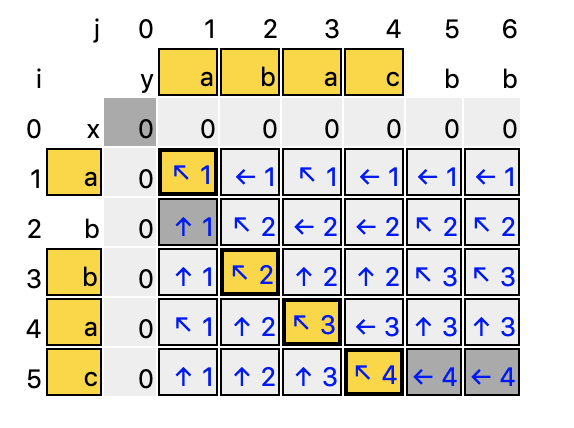
\includegraphics[height=4.5cm]{./grid.png}
\item
الگوریتمی از O(nk) ارائه دهید 
که تعداد راه‌های ساخت عدد n را با استفاده از سکه‌های $c_1, ..., c_k$ تومانی را با استفاده از O(n) خانه‌ی حافظه بشمارد. توجه کنید که از هر سکه نهایتا یک‌بار می‌توان استفاده کرد.

راه‌حل: $dp_{n,i}$ را تعریف می‌کنم تعداد روش‌هایی که می‌توان عدد n را با استفاده از i سکه اول تولید کرد. با توجه به ساختار سوال $dp_{n,i}$ از $dp_{n-c_i, i-1}$ و $dp_{n, i-1}$ محاسبه می‌شود. حال در نظر بگیرید که به جای یک آٰرایه‌ی دو بعدی از آرایه‌ی یک بعدی $dp_n$ استفاده کنیم. در این صورت به نظر می‌رسد که با تکه کد زیر می‌توان پاسخ بهینه را با حافظه‌ی $O(n)$ محاسبه کرد.

\begin{minted}{python}
for j = 1 -> k:
    for i = 1 -> n:
        if (i >= c[j])
            dp[i] = dp[i] + dp[i - c[j]]
\end{minted}

مشکل این کد این است که تضمینی وجود ندارد که $dp[i-c[j]]$ خودش در این مرحله بروزرسانی نشده باشد و ممکن است که او نیز با استفاده از سکه‌ی فعلی ساخته شده باشد. نکته سوال این است که هیچ لزومی وجود ندارد که dp از مقدار کم به زیاد بروزرسانی شود و می‌تواند از مقدار زیاد به کم نیز بروزرسانی شود. در این شرایط ایرادی که به الگوریتم وارد است دیگر پیش نخواهد آمد و درست عمل خواهد کرد. بنابراین تکه کد زیر پاسخ صحیح مسئله است.

\begin{minted}{python}
for j = 1 -> k:
    for i = n -> 1:
        if (i >= c[j])
            dp[i] = dp[i] + dp[i - c[j]]
\end{minted}ریتضمینی وجود نداردکتم ادعاtem
در یک  که ارخانه چوب‌بری عجیب برای اینک۱ وه یک تکه چوب را در یک مرحله به k تکه برش بزنند $c_k$ تومن پول گرفته می‌شود.
\begin{itemize}
    \item الگوریتمی از $O(n^2)$ ارائه دهید که یک تکه چوب را با کمترین خرج به n تکه تقسیم کند.
    % \item فرض کنید $c_k$ ها صعودی باشند. الگوریتمی از $O(nlogn)$ ارائه دهید. (این بخش امتیازی می‌باشد.)
\end{itemize}

راه‌حل: $dp_n$ را تعریف می‌کنم کمترین هزینه‌ای که باصرف آن می‌توان یک تکه چوب را به n تکه تبدیل کرد. در گام آخر قبل از رسیدن به n تکه $n-k+1$ تکه
داشته بودیم که با انجام یک برش k تایی به n تکه رسیده‌ایم. به این ترتیب با یک حلقه و بررسی تمامی حالت‌های ممکن می‌توان با صرف $O(n^2)$ مسئله را حل کرد.
\end{itemize}

\end{enumerate}

\end{document}
